\documentclass[12pt]{report}
\usepackage{amsmath}
\usepackage{latexsym}
\usepackage{amsfonts}
\usepackage[normalem]{ulem}
\usepackage{soul}
\usepackage{array}
\usepackage{amssymb}
\usepackage{extarrows}
\usepackage{graphicx}
\usepackage[backend=biber,
style=numeric,
sorting=none,
isbn=false,
doi=false,
url=false,
]{biblatex}\addbibresource{bibliography.bib}

\usepackage{subfig}
\usepackage{wrapfig}
\usepackage{wasysym}
\usepackage{enumitem}
\usepackage{adjustbox}
\usepackage{ragged2e}
\usepackage[svgnames,table]{xcolor}
\usepackage{tikz}
\usepackage{longtable}
\usepackage{changepage}
\usepackage{setspace}
\usepackage{hhline}
\usepackage{multicol}
\usepackage{tabto}
\usepackage{float}
\usepackage{multirow}
\usepackage{makecell}
\usepackage{fancyhdr}
\usepackage[toc,page]{appendix}
\usepackage[hidelinks]{hyperref}
\usetikzlibrary{shapes.symbols,shapes.geometric,shadows,arrows.meta}
\tikzset{>={Latex[width=1.5mm,length=2mm]}}
\usepackage{flowchart}\usepackage[paperheight=11.69in,paperwidth=8.27in,left=1.0in,right=0.97in,top=1.0in,bottom=1.0in,headheight=1in]{geometry}
\usepackage[utf8]{inputenc}
\usepackage[T1]{fontenc}
\TabPositions{0.5in,1.0in,1.5in,2.0in,2.5in,3.0in,3.5in,4.0in,4.5in,5.0in,5.5in,6.0in,}

\urlstyle{same}

\renewcommand{\_}{\kern-1.5pt\textunderscore\kern-1.5pt}

 %%%%%%%%%%%%  Set Depths for Sections  %%%%%%%%%%%%%%

% 1) Section
% 1.1) SubSection
% 1.1.1) SubSubSection
% 1.1.1.1) Paragraph
% 1.1.1.1.1) Subparagraph


\setcounter{tocdepth}{5}
\setcounter{secnumdepth}{5}


 %%%%%%%%%%%%  Set Depths for Nested Lists created by \begin{enumerate}  %%%%%%%%%%%%%%


\setlistdepth{9}
\renewlist{enumerate}{enumerate}{9}
		\setlist[enumerate,1]{label=\arabic*)}
		\setlist[enumerate,2]{label=\alph*)}
		\setlist[enumerate,3]{label=(\roman*)}
		\setlist[enumerate,4]{label=(\arabic*)}
		\setlist[enumerate,5]{label=(\Alph*)}
		\setlist[enumerate,6]{label=(\Roman*)}
		\setlist[enumerate,7]{label=\arabic*}
		\setlist[enumerate,8]{label=\alph*}
		\setlist[enumerate,9]{label=\roman*}

\renewlist{itemize}{itemize}{9}
		\setlist[itemize]{label=$\cdot$}
		\setlist[itemize,1]{label=\textbullet}
		\setlist[itemize,2]{label=$\circ$}
		\setlist[itemize,3]{label=$\ast$}
		\setlist[itemize,4]{label=$\dagger$}
		\setlist[itemize,5]{label=$\triangleright$}
		\setlist[itemize,6]{label=$\bigstar$}
		\setlist[itemize,7]{label=$\blacklozenge$}
		\setlist[itemize,8]{label=$\prime$}



 %%%%%%%%%%%%  Header here  %%%%%%%%%%%%%%


\pagestyle{fancy}
\fancyhf{}
\cfoot{ \begin{FlushRight}
\ \  
\end{FlushRight}}
\renewcommand{\headrulewidth}{0pt}
\setlength{\topsep}{0pt}\setlength{\parindent}{0pt}

 %%%%%%%%%%%%  This sets linespacing (verticle gap between Lines) Default=1 %%%%%%%%%%%%%%


\renewcommand{\arraystretch}{1.3}

\title{Software Requirements Specification for DayGame}
\author{Yorgos Basioukas, Kapoutselis Christos, Moschopoulos Apostolis, \\
Papadopoulou Athanasia, Sarafoglou Marina, Spiridopoulos Konstantinos, \\
Dadidis Mitrofanos, Tsirpanis Theodoris}
\date{}


%%%%%%%%%%%%%%%%%%%% Document code starts here %%%%%%%%%%%%%%%%%%%%



\begin{document}

\maketitle
\setlength{\parskip}{2.04pt}
\par

\chapter{Group 7}\par


\vspace{\baselineskip}

\vspace{\baselineskip}

\vspace{\baselineskip}

\vspace{\baselineskip}

\vspace{\baselineskip}

\vspace{\baselineskip}

\vspace{\baselineskip}

\vspace{\baselineskip}

\vspace{\baselineskip}

\vspace{\baselineskip}

\vspace{\baselineskip}


%%%%%%%%%%%%%%%%%%%% Table No: 1 Group 7 team starts here %%%%%%%%%%%%%%%%%%%%


\begin{table}[H]
 			\centering
\begin{tabular}{p{2.77in}p{1.04in}}
\hline
%row no:1
\multicolumn{1}{p{2.77in}}{\textit{Name}} & 
\multicolumn{1}{p{1.04in}}{\textit{ID}} \\
\hhline{~~}
%row no:2
\multicolumn{1}{p{2.77in}}{Basileiadis Anestis} & 
\multicolumn{1}{p{1.04in}}{dai19272} \\
\hhline{~~}
%row no:3
\multicolumn{1}{p{2.77in}}{Kapoutselis Christos} & 
\multicolumn{1}{p{1.04in}}{it14234} \\
\hhline{~~}
%row no:4
\multicolumn{1}{p{2.77in}}{Moschopoulos Apostolis} & 
\multicolumn{1}{p{1.04in}}{dai19104} \\
\hhline{~~}
%row no:5
\multicolumn{1}{p{2.77in}}{Basioukas Yorgos} & 
\multicolumn{1}{p{1.04in}}{dai19174} \\
\hhline{~~}
%row no:6
\multicolumn{1}{p{2.77in}}{Dadidis Mitrofanos} & 
\multicolumn{1}{p{1.04in}}{dai19011} \\
\hhline{~~}
%row no:7
\multicolumn{1}{p{2.77in}}{Papadopoulos Dimitris} & 
\multicolumn{1}{p{1.04in}}{dai17096} \\
\hhline{~~}
%row no:8
\multicolumn{1}{p{2.77in}}{Papadopoulou Athanasia} & 
\multicolumn{1}{p{1.04in}}{dai19091} \\
\hhline{~~}
%row no:9
\multicolumn{1}{p{2.77in}}{Sarafoglou Marina} & 
\multicolumn{1}{p{1.04in}}{dai19080} \\
\hhline{~~}
%row no:10
\multicolumn{1}{p{2.77in}}{Spiridopoulos Konstantinos} & 
\multicolumn{1}{p{1.04in}}{dai19106} \\
\hhline{~~}
%row no:11
\multicolumn{1}{p{2.77in}}{Tsirpanis Theodoris} & 
\multicolumn{1}{p{1.04in}}{dai19090} \\
\hhline{~~}

\end{tabular}
 \end{table}


%%%%%%%%%%%%%%%%%%%% Table No: 1 Group 7 team ends here %%%%%%%%%%%%%%%%%%%%


\vspace{\baselineskip}

\vspace{\baselineskip}

\vspace{\baselineskip}
Instructor: Apostolos Ampatzoglou, Alexander Chatzigeorgiou \par

Course: Software Engineering


 %%%%%%%%%%%%  This Produces Table Of Contents %%%%%%%%%%%%%%

\tableofcontents
\addcontentsline{toc}{chapter}{Contents}

\vspace{\baselineskip}

\vspace{\baselineskip}

\vspace{\baselineskip}

\vspace{\baselineskip}

\vspace{\baselineskip}
\section*{Revision history}
\addcontentsline{toc}{section}{Revision history}


%%%%%%%%%%%%%%%%%%%% Table No: 2 Revision starts here %%%%%%%%%%%%%%%%%%%%


\begin{table}[H]
 			\centering
\begin{tabular}{p{2.26in}p{0.84in}p{2.03in}p{0.57in}}
\hline
%row no:1
\multicolumn{1}{|p{2.26in}}{\Centering \textbf{Name}} & 
\multicolumn{1}{|p{0.84in}}{\Centering \textbf{Date}} & 
\multicolumn{1}{|p{2.03in}}{\Centering \textbf{Reason}} & 
\multicolumn{1}{|p{0.57in}|}{\Centering \textbf{Version}} \\
\hhline{----}
%row no:2
\multicolumn{1}{|p{2.26in}}{Yorgos Basioukas} & 
\multicolumn{1}{|p{0.84in}}{\Centering 14/3/2020} & 
\multicolumn{1}{|p{2.03in}}{\Centering Created Document} & 
\multicolumn{1}{|p{0.57in}|}{\Centering \textbf{0.1}} \\
\hhline{----}
%row no:3
\multicolumn{1}{|p{2.26in}}{Yorgos Basioukas} & 
\multicolumn{1}{|p{0.84in}}{\Centering 14/3/2020} & 
\multicolumn{1}{|p{2.03in}}{\Centering Added Table of Contents and Revision} & 
\multicolumn{1}{|p{0.57in}|}{\Centering \textbf{0.2}} \\
\hhline{----}
%row no:4
\multicolumn{1}{|p{2.26in}}{Kapoutselis Christos \par Moschopoulos Apostolis  \par Papadopoulou Athanasia \par Sarafoglou Marina  \par Spiridopoulos Konstantinos \par Tsirpanis Theodoris } & 
\multicolumn{1}{|p{0.84in}}{\Centering 17/3/2020 \par } & 
\multicolumn{1}{|p{2.03in}}{\Centering Added\ Purpose,   \par \Centering Document Conventions, Intended Audience, \par \Centering  Product Scope, \par \Centering and Overall Description Section} & 
\multicolumn{1}{|p{0.57in}|}{\Centering \textbf{0.3}} \\
\hhline{----}
%row no:5
\multicolumn{1}{|p{2.26in}}{Moschopoulos Apostolis  \par Yorgos Basioukas \par Papadopoulou Athanasia \par Sarafoglou Marina  \par Spiridopoulos Konstantinos} & 
\multicolumn{1}{|p{0.84in}}{\Centering 18/3/2020} & 
\multicolumn{1}{|p{2.03in}}{\Centering Added Functional Requirements} & 
\multicolumn{1}{|p{0.57in}|}{\Centering \textbf{0.4}} \\
\hhline{----}
%row no:6
\multicolumn{1}{|p{2.26in}}{Kapoutselis Christos \par Moschopoulos Apostolis  \par Yorgos Basioukas \par Dadidis Mitrofanos \par Papadopoulou Athanasia \par Sarafoglou Marina} & 
\multicolumn{1}{|p{0.84in}}{\Centering 20/3/2020} & 
\multicolumn{1}{|p{2.03in}}{\Centering Added Shop and Update Task Use Cases \par } & 
\multicolumn{1}{|p{0.57in}|}{\Centering \textbf{0.5}} \\
\hhline{----}
%row no:7
\multicolumn{1}{|p{2.26in}}{Yorgos Basioukas \par Papadopoulou Athanasia} & 
\multicolumn{1}{|p{0.84in}}{\Centering 24/3/2020} & 
\multicolumn{1}{|p{2.03in}}{\Centering Added Boss Battle Use Case} & 
\multicolumn{1}{|p{0.57in}|}{\Centering \textbf{0.6}} \\
\hhline{----}
%row no:8
\multicolumn{1}{|p{2.26in}}{Kapoutselis Christos \par Moschopoulos Apostolis  \par Yorgos Basioukas \par Papadopoulou Athanasia \par Sarafoglou Marina \par Spiridopoulos Konstantinos} & 
\multicolumn{1}{|p{0.84in}}{\Centering 26/3/2020} & 
\multicolumn{1}{|p{2.03in}}{\Centering Reviewed Use Cases} & 
\multicolumn{1}{|p{0.57in}|}{\Centering \textbf{0.7}} \\
\hhline{----}
%row no:9
\multicolumn{1}{|p{2.26in}}{Kapoutselis Christos \par Moschopoulos Apostolis  \par Yorgos Basioukas} & 
\multicolumn{1}{|p{0.84in}}{\Centering 26/3/2020} & 
\multicolumn{1}{|p{2.03in}}{\Centering Added Non-Functional Requirements} & 
\multicolumn{1}{|p{0.57in}|}{\Centering \textbf{0.8}} \\
\hhline{----}
%row no:10
\multicolumn{1}{|p{2.26in}}{Kapoutselis Christos \par Moschopoulos Apostolis  \par Yorgos Basioukas \par Papadopoulou Athanasia \par Sarafoglou Marina \par Spiridopoulos Konstantinos} & 
\multicolumn{1}{|p{0.84in}}{\Centering 27/3/2020} & 
\multicolumn{1}{|p{2.03in}}{\Centering Added References, Definitions, Acronyms and Abbreviations,  \par \Centering Product Functions and Appendix} & 
\multicolumn{1}{|p{0.57in}|}{\Centering \textbf{0.9}} \\
\hhline{----}
%row no:11
\multicolumn{1}{|p{2.26in}}{Kapoutselis Christos \par Moschopoulos Apostolis  \par Yorgos Basioukas \par Papadopoulou Athanasia \par Sarafoglou Marina} & 
\multicolumn{1}{|p{0.84in}}{\Centering 29/3/2020} & 
\multicolumn{1}{|p{2.03in}}{\Centering Added Product in a Box, \par \Centering Use Case Diagram, \par \Centering User-Goal Diagram} & 
\multicolumn{1}{|p{0.57in}|}{\Centering \textbf{1.0}} \\
\hhline{----}
%row no:12
\multicolumn{1}{|p{2.26in}}{Yorgos Basioukas} & 
\multicolumn{1}{|p{0.84in}}{\Centering 19/4/2020} & 
\multicolumn{1}{|p{2.03in}}{\Centering Created LaTeX version of this document} & 
\multicolumn{1}{|p{0.57in}|}{\Centering \textbf{1.1}} \\
\hhline{----}

\end{tabular}
 \end{table}


%%%%%%%%%%%%%%%%%%%% Table No: 2 Revision ends here %%%%%%%%%%%%%%%%%%%%


\vspace{\baselineskip}

\vspace{\baselineskip}

\vspace{\baselineskip}

\vspace{\baselineskip}

\vspace{\baselineskip}

\vspace{\baselineskip}

\vspace{\baselineskip}

\vspace{\baselineskip}

\vspace{\baselineskip}\section*{1. Introduction }
\addcontentsline{toc}{section}{1. Introduction }
\subsection*{1.1 Purpose}
\addcontentsline{toc}{subsection}{1.1 Purpose}

\vspace{\baselineskip}
The purpose of this document is to provide a detailed description of the functional and non-functional requirements of the desktop application DayGame. It will explain the purpose and features of the software, the interfaces of the software, what the software will do and the constraints under which it must operate. This document is intended for users of the software and also potential developers.\par

\subsection*{1.2 Document Conventions }
\addcontentsline{toc}{subsection}{1.2 Document Conventions }

\vspace{\baselineskip}
This Document was created based on the IEEE standard 830 for System Requirement Specification Documents. \par

\subsection*{1.3 Intended Audience }
\addcontentsline{toc}{subsection}{1.3 Intended Audience }

\vspace{\baselineskip}
This document is intended to be used by members of the project team that will implement and verify the correct functioning of the system. \par

\subsection*{1.4 Product Scope}
\addcontentsline{toc}{subsection}{1.4 Product Scope}

\vspace{\baselineskip}
DayGame is a desktop application that focuses on managing tasks in an interactive way using elements from role-playing games, while tracking everyday tasks and motivating users to complete them in exchange for virtual rewards. \par


\newpage

\vspace{\baselineskip}\subsection*{1.5 References }
\addcontentsline{toc}{subsection}{1.5 References }
\textbf{IEEE Recommended Practice for Software Requirements Specifications:}\par

\href{http://www.cse.msu.edu/~cse870/IEEEXplore-SRS-template.pdf}{\textcolor[HTML]{1155CC}{\ul{http://www.cse.msu.edu/$ \sim $ cse870/IEEEXplore-SRS-template.pdf}}}\par


\vspace{\baselineskip}
\textbf{IEEE SRS summary and explanation}\par

\href{https://www.cin.ufpe.br/~if716/arquivos20162/03-IEEE-830}{\textcolor[HTML]{1155CC}{\ul{https://www.cin.ufpe.br/$ \sim $ if716/arquivos20162/03-IEEE-830}}}\par


\vspace{\baselineskip}
\textbf{DayGame’s GitHub page:}\par

\href{https://github.com/teo-tsirpanis/DayGame}{\textcolor[HTML]{1155CC}{\ul{https://github.com/teo-tsirpanis/DayGame}}}\par


\vspace{\baselineskip}
\textbf{MIT License :}\par

\href{https://opensource.org/licenses/MIT}{\textcolor[HTML]{1155CC}{\ul{https://opensource.org/licenses/MIT}}}\par


\vspace{\baselineskip}
\textbf{SRS template and Use Case tables provided by instructors}\par


\vspace{\baselineskip}
\textbf{Software development with the use of ICONIX methodology (Greek)}\par

\href{http://users.uom.gr/~achat/AdvSoftEng/ICONIX_eBook.pdf}{\textcolor[HTML]{1155CC}{\ul{http://users.uom.gr/$ \sim $ achat/AdvSoftEng/ICONIX\_eBook.pdf}}}\par


\vspace{\baselineskip}
\textbf{Software Requirements Specification for Gephi}\par

\href{https://gephi.org/users/gephi_srs_document.pdf}{\textcolor[HTML]{1155CC}{\ul{https://gephi.org/users/gephi\_srs\_document.pdf}}}\par


\vspace{\baselineskip}
\textbf{Software Requirements Specification for TimeTracker 2.0}\par

\href{https://trello-attachments.s3.amazonaws.com/58c0dc2106266ad55c4a3486/58c65f5a171e24879e1e0d02/d94c2d78161d54c8779a4ffdeba0cff9/srs.pdf}{\textcolor[HTML]{1155CC}{\ul{https://trello-attachments.s3.amazonaws.com/58c0dc2106266ad55c4a3486/58c65f5a171e24879e1e0d02/d94c2d78161d54c8779a4ffdeba0cff9/srs.pdf}}}\par


\vspace{\baselineskip}
\textbf{Software Requirements Specification for AASTU Digital Information Desk }\par

\href{https://www.studocu.com/row/document/addis-ababa-university/software-engineering/mandatory-assignments/ieee-830-1998-standard-srs-document/1981874/view}{\textcolor[HTML]{1155CC}{\ul{https://www.studocu.com/row/document/addis-ababa-university/software-engineering/mandatory-assignments/ieee-830-1998-standard-srs-document/1981874/view}}}\par


\vspace{\baselineskip}
\textbf{Software requirements specification Wikipedia}\par

\href{https://en.wikipedia.org/wiki/Software_requirements_specification}{\textcolor[HTML]{1155CC}{\ul{https://en.wikipedia.org/wiki/Software\_requirements\_specification}}}\par


\newpage

\vspace{\baselineskip}\subsection*{1.6 Definitions, Acronyms and Abbreviations}
\addcontentsline{toc}{subsection}{1.6 Definitions, Acronyms and Abbreviations}
\textbf{\textit{RPG}}: Role Playing Game\par

\textbf{\textit{UI}}: User Interface\par

\textbf{\textit{UC}}: Use Case\par

\textbf{\textit{FAQ}}: Frequently Asked Questions\par


\vspace{\baselineskip}
\textbf{\textit{Actor}}:\ A user whose defined  user goal and is fulfilled by the \textit{System}.\par

\textbf{\textit{Appearance}}: Depending on \textit{Gender,} \textit{Appearance }is a visual representation of the\textit{ Character} or the \textit{Boss.}\par

\textbf{\textit{Armor}}: \textit{Item} that adds \textit{Defence} when \textit{Equipped}.\par

\textbf{\textit{Attack}}: \textit{Damage }being done from the \textit{Character }or the\textit{ Boss}.\par

\textbf{\textit{Bag}}: Stores \textit{Consumable Items} from the \textit{Inventory }that the \textit{Character} can use in the \textit{Boss Battles}. There is limited space. Can not be changed during the \textit{Boss Battles.}\par

\textbf{\textit{Boss}}: \textcolor[HTML]{222222}{A \textit{System}-controlled enemy.}\par

\textbf{\textit{\textcolor[HTML]{222222}{Boss Battle}}}: \textcolor[HTML]{222222}{A digital fight between a\textit{ Boss }and a \textit{Character.}}\par

\textbf{\textit{Character}}: An \textit{Actor.}\par

\textbf{\textit{Complete Tasks}}: Finished \textit{Tasks}. \textit{Character} wins \textit{in-game balance} and \textit{experience points. }For $``$\textit{Dailies}$"$  or $``$\textit{To-Dos$"$ }, the system also checks whether the \textit{Due Date} set by the user has not expired.\par

\textbf{\textit{Consumable\ Items:  }}\textit{Items} that can be used once. There are two types. \textit{Spells} and \textit{Potions.}\par

\textbf{\textit{Damage}}: It refers to an integer amount of \textit{Hit }or \textit{Life points }being lost.\par

\textbf{\textit{Defence}}: It refers to an integer amount of points that is negated from \textit{Damage }dealt by a \textit{Boss}.\par

\textbf{\textit{Difficulty: }}There are four types. Easy, Medium, Hard, DARK SOULS used in creating a \textit{Task }with different rewards in \textit{Experience Points} and \textit{In-game balance }when \textit{Completed}.\par

\textbf{\textit{Due Date}}: Only applicable to $``$\textit{Dailies$"$ } and $``$\textit{To-Dos$"$ }. The date is specified by a number in the calendar.\par

\textbf{\textit{Entities}}: The \textit{Character} and the\textit{ Boss}.\par

\textbf{\textit{\textcolor[HTML]{222222}{Equip Items}}}\textcolor[HTML]{222222}{: User can \textit{Equip Items} to the \textit{Character} that increases his \textit{Stats}, in order to have greater chances of winning in \textit{Boss Battles}. Can not be done during the\textit{ Boss Battle.}There are limited slots, for example 1 for \textit{Weapon} and 1 for \textit{Armor.}}\par

\textbf{\textit{Equippable Items}}: Purchased \textit{Items} that can be \textit{Equipped} to the \textit{Character}. There are two types. \textit{Weapons} and \textit{Armor.}\par

\textbf{\textit{Experience Bar}}: The visual representation of \textit{Experience Points }in a bar. \par

\textbf{\textit{Experience points}}: Indicates the amount of integer points achieved by \textit{Completing} \textit{Tasks or }winning\textit{ Boss Battles}. Reaching a specific amount of points increases the \textit{Character’s Level. }After the \textit{character Levels Up }the points are reset to zero\textit{.}\par

\textbf{\textit{Frequently Asked Questions}}: A set of questions and answers made by the developers for easier program use and problem solving.\par

\textbf{\textit{Gender}}: Male and Female options.\par

\newpage
\textbf{\textit{Hit points}}: \textit{Hit points} are used only in \textit{Boss Battles}\par

\begin{itemize}
	\item For\textit{ Characters}: A copy of current \textit{Life points}\par

	\item For \textit{Bosses}: An integer amount of points \textcolor[HTML]{222222}{that indicates the \textit{Boss’ }}continued ability to function during the\textit{ battle}
\end{itemize}\par

\vspace{\baselineskip}
\textbf{\textit{Hit point regain}}: An integer amount of points added to\textit{ Hit points }\par

\textbf{\textit{In-game balance}}: Digital currency that can be spend on the \textit{Shop}. It can be acquired through \textit{Completing Tasks} or \textit{Boss Battles.}\par

\textbf{\textit{Items}}: A set of digital products that can be purchased from the \textit{Shop} with \textit{In-game balance. }Different kind of \textit{Items} have different \textit{stats.}\par

\textbf{\textit{Inventory: }}Placeholder for all Items purchased at the \textit{Shop}. \par

\textbf{\textit{Item category}}: Armor, Weapons, Spells and Potions.\par

\textbf{\textit{Jackpot}}: Earning double amount of \textit{rewards }after completing a \textit{task}.\par

\textbf{\textit{Level}}: An integer number that shows the rate of game progression and difficulty\par

\textbf{\textit{Level up}}: When the character gets all required \textit{Experience Points} it \textit{Levels Up}. With this process it regains all\textit{ Life points }and E\textit{xperience Points} are reset to zero. In addition you can increase a \textit{Stat} type of \textit{Damage} or \textit{Defence.}\par

\textbf{\textit{Life Bar}}: The visual representation of \textit{Life points }in a bar. \par

\textbf{\textit{Life points}}: An integer amount of points \textcolor[HTML]{222222}{that indicates the \textit{Character’s} continued ability to function out of\textit{ Boss Battles.}}The character dies after it reaches 0 points or less, losing all progress.\par

\textbf{\textit{Luck}}: A \textit{stat }that defines the possibility to get a \textit{jackpot} after completing a task.\par

\textbf{\textit{Navigate Menu}}:The main menu of the program which is always locked in the UI when user interacts with the game.\par

\textbf{\textit{Procrastinate Tasks}}: Unfinished \textit{Tasks}. \textit{Character} loses \textit{in-game balance}, \textit{experience points} and \textit{Life points.} For $``$Dailies$"$  or $``$To-Dos$"$ , the system also checks whether the time frame set by the user has expired \par

\textbf{\textit{Potions}}: \textit{Consumable Items} that \textit{regains hit points }to the \textit{character}.\par

\textbf{\textit{Quest Log}}: The main page where the user lands after \textit{character} selection or creation. It contains all tasks and their functions.\par

\textbf{\textit{Rewards}}: There are two types. classic reward multiplied by one and \textit{jackpot.}\par

\textbf{\textit{Shop}}: The place where you can buy\textit{ items.}\par

\textbf{\textit{Spells}}: \textit{Consumable items} that deal more \textit{Damage} to \textit{Bosses}.\par

\textbf{\textit{Start Page}}: The window when the user opens the program\par

\textbf{\textit{Stats}}\textit{: }Types are \textit{Damage}, \textit{Defence, Hit points, Luck.}\par

\textbf{\textit{System}}: \textcolor[HTML]{222222}{A group of interacting or interrelated entities that form a unified whole}\par

\textbf{\textit{Tasks}}\textit{:} A \textit{Task }is defined as an achievement to be reached. It is set by the user and falls under the following categories\par

\begin{itemize}
	\item Dailies: \textit{Tasks }that check completion on week-days, scheduled by the user\par

	\item Habits: \textit{Tasks }that refresh every day\par

	\item To-Dos: \textit{Tasks }that check completion on specific days
\end{itemize}\par

\textbf{\textit{Turn Based Battle}}: Turn based battle is where the \textit{Actor} and the \textit{Boss} are playing with turns. The \textit{Actor} is making a move and the \textit{Boss} is waiting for his own.\par

\textbf{\textit{\textcolor[HTML]{222222}{Unequip Items}}}\textcolor[HTML]{222222}{: User can \textit{unequip items} from the \textit{character} in order to \textit{equip} better \textit{items}. Can not be done during the\textit{ Boss Battles}. }\par

\textbf{\textit{Visibility}}: All\textit{ Items} are visible at first. User can select to apply a filter for a specific \textit{item category} that hides the rest of the \textit{Items} not belonging to that category.\par

\textbf{\textit{Weapon}}: Item that increases \textit{Damage} dealt to \textit{Bosses} when equipped.\par


\vspace{\baselineskip}

\vspace{\baselineskip}
\section*{2. Overall Description}
\addcontentsline{toc}{section}{2. Overall Description}
\subsection*{2.1 Product Perspective}
\addcontentsline{toc}{subsection}{2.1 Product Perspective}
DayGame is a gamified task management application, that provides users the ability to engage with their everyday tasks and habits. By adding RPG elements, the application intends to add significance to ordinary tasks and thus make them more appealing and interesting. The users can create their own character, select or add tasks, buy items using in-game balance and battle opponents. The product has been developed to run on Windows environments. \par


\vspace{\baselineskip}
\subsection*{2.2 Product Functions }
\addcontentsline{toc}{subsection}{2.2 Product Functions }
This section describes concisely all the product functions. For a more general description see Appendix A\par


\vspace{\baselineskip}
Start Page: \par

\begin{itemize}
	\item Choose Character: User chooses between their created characters. Data shown are the character’s level, name and appearance\par

	\item Create Character: Opens a form and user chooses name and gender\par

	\item Delete Character : Shows a confirmation message and if it is affirmative then it deletes the selected character and shows the start page, else it shows the start page
\end{itemize}\par


\vspace{\baselineskip}
Navigate Menu:\par

\begin{itemize}
	\item Quest Log: Displays the Task Log menu \par

	\item Shop: Displays Shop menu\par

	\item Inventory: Displays Inventory menu\par

	\item Battle: Displays the Boss Battle menu\par

	\item Help: Displays FAQ and feedback menu
\end{itemize}\par


\vspace{\baselineskip}
\vspace{\baselineskip}
Character Profile:\par

\begin{itemize}
	\item Contains character’s data\par

\begin{itemize}
	\item Character Appearance \par

	\item Character Name\par

	\item Experience Bar\par

	\item Life Bar\par

	\item Character Level\par

	\item In Game Balance\par
\end{itemize}
\end{itemize}

\vspace{\baselineskip}
Quest Log:\par

\begin{itemize}
	\item Task Log: A log containing three types of ongoing tasks: Habits, To-Dos, Dailies\par

	\item Add task: User creates a task and it is then stored into the Task Log. User needs to write the name of the task, the Task Type, its Difficulty and the Due Date, if possible\par

	\item Update Task\par

\begin{itemize}
	\item Complete Task: Marks a task as completed \par

	\item Procrastinate Task: Marks a task as unfinished\par

	\item Level Up if preconditions are met\par


\end{itemize}
	\item Delete Task: Deletes task from the log\par

	\item Drag And Drop Tasks: The ability to switch tasks placement
\end{itemize}\par


\vspace{\baselineskip}
Shop: \par

\begin{itemize}
	\item Item filter: Changes item visibility based on the users choice\par

	\item View Item: Opens window that shows the item’s stats and description\par

	\item Buy Item: Adds item in the user’s inventory and updates the user’s gold balance
\end{itemize}\par


\vspace{\baselineskip}
Inventory:\par

\begin{itemize}
	\item Item filter: Changes item visibility based on the users choice\par

	\item View Item: Opens window that shows the item’s stats and description\par

	\item Equip Item: Equips the selected item to the character.\par

	\item Unequip Item: Unequips the selected item from the character
\end{itemize}\par


Boss Battle: \par

\begin{itemize}
	\item Turn based battle system\par

	\item Selection menu: Attack, Spells, Potions\par

\begin{itemize}
	\item Attack: The user’s character performs an attack on the boss\par

	\item Spells: The user’s character performs a special attack on the boss using an item\par

	\item Potions: The user’s character performs a self-healing ability using an item \par


\end{itemize}
	\item Use Items: uses a consumable item from the bag \par

	\item Boss Functions: Attacks after user’s turn\par

	\item Character deals damage depending on level and items that add to the overall stats\par

	\item Boss deals damage depending on character’s level
\end{itemize}\par


\vspace{\baselineskip}

\vspace{\baselineskip}

\vspace{\baselineskip}

\vspace{\baselineskip}
Character Death:\par

\begin{itemize}
	\item Shows appropriate message and character loses one level
\end{itemize}\par


\vspace{\baselineskip}
Help:\par

\begin{itemize}
	\item Contains a Frequently Asked Questions form
\end{itemize}\par

\begin{itemize}
	\item Feedback: Shows a text field for the user to give feedback or report a bug
\end{itemize}\par


\vspace{\baselineskip}
Autosave:\par

\begin{itemize}
	\item System saves characters’ data and progress in a text file.\par

	\item Read: every time a user chooses a character, the system loads the appropriate file from the saved log directory\par

	\item Write: System writes into a text file all progress done in the game and stores it to a saved log directory
\end{itemize}\par


\newpage
{\fontsize{14pt}{16.8pt}\selectfont Use Case Diagram:\par}\par



%%%%%%%%%%%%%%%%%%%% Figure No: 1 Use Case Diagram starts here %%%%%%%%%%%%%%%%%%%%

\begin{figure}[H]
	\begin{Center}
		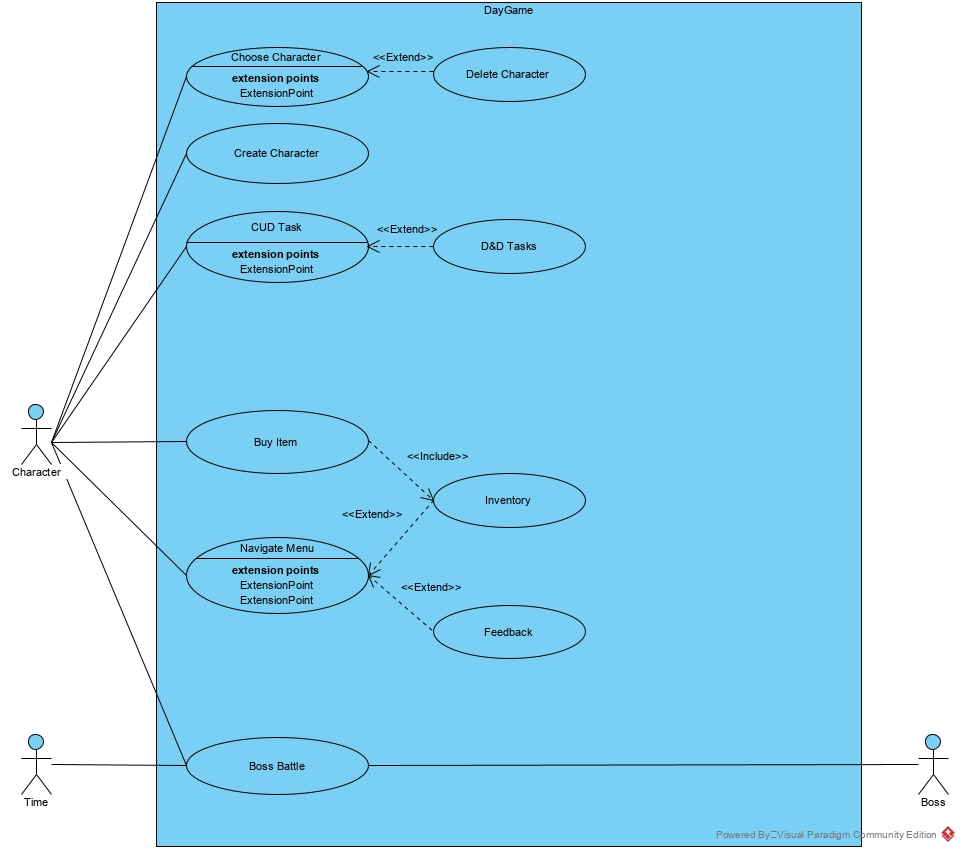
\includegraphics[width=6.3in,height=5.58in]{./media/image1.jpg}
	\end{Center}
\end{figure}


%%%%%%%%%%%%%%%%%%%% Figure No: 1 Use Case Diagram Ends here %%%%%%%%%%%%%%%%%%%%

\newpage
{\fontsize{14pt}{16.8pt}\selectfont User-Goal Diagram:\par}\par



%%%%%%%%%%%%%%%%%%%% Table No: 3 User Goal Diagram starts here %%%%%%%%%%%%%%%%%%%%


\begin{table}[H]
 			\centering
\begin{tabular}{p{2.95in}p{2.95in}}
\hline
%row no:1
\multicolumn{1}{|p{2.95in}}{\Centering \textbf{User}} & 
\multicolumn{1}{|p{2.95in}|}{\Centering \textbf{Goal}} \\
\hhline{--}
%row no:2
\multicolumn{1}{|p{2.95in}}{\Centering Character} & 
\multicolumn{1}{|p{2.95in}|}{\Centering Choose Character \par \Centering Create Character \par \Centering Delete Character \par \Centering Navigate Menu \par \Centering CUD Tasks \par \Centering D$\&$D Tasks \par \Centering Buy Item \par \Centering Inventory \par \Centering Feedback \par \Centering Boss Battle} \\
\hhline{--}
%row no:3
\multicolumn{1}{|p{2.95in}}{\Centering Boss} & 
\multicolumn{1}{|p{2.95in}|}{\Centering Boss Battle} \\
\hhline{--}
%row no:4
\multicolumn{1}{|p{2.95in}}{\Centering Time} & 
\multicolumn{1}{|p{2.95in}|}{\Centering Boss Battle} \\
\hhline{--}

\end{tabular}
 \end{table}


%%%%%%%%%%%%%%%%%%%% Table No: 3 User Goal Diagram ends here %%%%%%%%%%%%%%%%%%%%


\vspace{\baselineskip}


\subsection*{2.3 User Classes and Characteristics}
\addcontentsline{toc}{subsection}{2.3 User Classes and Characteristics}
Anyone that desires to organize their time.There are no specific characteristics required for use.\par

\subsection*{2.4 Operating Environment\  }
\addcontentsline{toc}{subsection}{2.4 Operating Environment\  }
DayGame will be able to run on:\par

\begin{itemize}
	\item Windows 7 SP1+ on both architectures (x64, x86)\par

	\item Windows\  8.1 on both architectures (x64, x86)\par

	\item Windows 10 Version 1607+ on both architectures (x64, x86)
\end{itemize}\par

\subsection*{2.5 Design and implementation constraints}
\addcontentsline{toc}{subsection}{2.5 Design and implementation constraints}
\begin{itemize}
	\item System requirements from a casual web browsing computer are enough to run the program\par

	\item Quantitatively data are subject to change and sometimes are not defined in this document. Testers will be responsible for this job
\end{itemize}\par

\subsection*{2.6 Assumptions and Dependencies}
\addcontentsline{toc}{subsection}{2.6 Assumptions and Dependencies}
\begin{itemize}
	\item The users have sufficient knowledge of operating a computer\par

	\item The\ users know the English language, as the user interface will be provided in English  
\end{itemize}\par
\newpage
\section*{3. Specific Requirements}
\addcontentsline{toc}{section}{3. Specific Requirements}
\subsection*{3.1 Functional Requirements}
\addcontentsline{toc}{subsection}{3.1 Functional Requirements}
\subsubsection*{3.1.1 Boss Battle}
\addcontentsline{toc}{subsubsection}{3.1.1 Boss Battle}


%%%%%%%%%%%%%%%%%%%% Table No: 4 Boss Battle starts here %%%%%%%%%%%%%%%%%%%%


{
\setlength\extrarowheight{3pt}
\begin{longtable}{p{0.51in}p{1.5in}p{-0.13in}p{3.62in}}

\endfirsthead
\multicolumn{4}{c}{\textit{continued from previous page}}\\ \hline
\endhead
\multicolumn{4}{r}{\textit{continued on next page}} \\
\endfoot
\endlastfoot%row no:1
\multicolumn{3}{p{\dimexpr1.88in+4\tabcolsep\relax}}{\cellcolor[HTML]{BFBFBF}\textbf{Use Case Name}} & 
\multicolumn{1}{p{3.62in}}{Boss Battle (UC-10)} \\
\hhline{~~~~}
%row no:2
\multicolumn{4}{p{\dimexpr5.5in+6\tabcolsep\relax}}{\cellcolor[HTML]{BFBFBF}\textbf{Brief Description}} \\
\hhline{~~~~}
%row no:3
\multicolumn{4}{p{\dimexpr5.5in+6\tabcolsep\relax}}{The use case is called after the precondition is met to fight a strong boss. User ought to have completed enough tasks by that time, in order to get items to increase their chances of winning. If the user loses, they will have to fight the boss with the same stats again} \\
\hhline{~~~~}
%row no:4
\multicolumn{4}{p{\dimexpr5.5in+6\tabcolsep\relax}}{\cellcolor[HTML]{BFBFBF}\textbf{Flow of Events}} \\
\hhline{~~~~}
%row no:5
\multicolumn{4}{p{\dimexpr5.5in+6\tabcolsep\relax}}{\textbf{Basic Flow}} \\
\hhline{~~~~}
%row no:6
\multicolumn{1}{p{0.51in}}{\Centering 1} & 
\multicolumn{3}{p{\dimexpr4.99in+4\tabcolsep\relax}}{After the precondition is met. System shows UI-12 $``$Boss Battle$"$ } \\
\hhline{~~~~}
%row no:7
\multicolumn{1}{p{0.51in}}{\Centering 2} & 
\multicolumn{3}{p{\dimexpr4.99in+4\tabcolsep\relax}}{User makes the first move by choosing either $``$Attack$"$ , $``$Spells$"$  or $``$Potions$"$ } \\
\hhline{~~~~}
%row no:8
\multicolumn{1}{p{0.51in}}{\Centering 3} & 
\multicolumn{3}{p{\dimexpr4.99in+4\tabcolsep\relax}}{User selects $``$Attack$"$ } \\
\hhline{~~~~}
%row no:9
\multicolumn{1}{p{0.51in}}{\Centering 4} & 
\multicolumn{3}{p{\dimexpr4.99in+4\tabcolsep\relax}}{User\ deals\ damage to the boss. System shows message $"$ +x   damage$"$ , x being the number of damage that the user can attack with.} \\
\hhline{~~~~}
%row no:10
\multicolumn{1}{p{0.51in}}{\Centering 5} & 
\multicolumn{3}{p{\dimexpr4.99in+4\tabcolsep\relax}}{\  System updates the Hit points of the boss} \\
\hhline{~~~~}
%row no:11
\multicolumn{1}{p{0.51in}}{\Centering 6} & 
\multicolumn{3}{p{\dimexpr4.99in+4\tabcolsep\relax}}{Boss\ makes\ second move that deals damage to the user. System shows message $"$ +x   damage$"$ , x being the number of damage that the boss attacks with} \\
\hhline{~~~~}
%row no:12
\multicolumn{1}{p{0.51in}}{\Centering 7} & 
\multicolumn{3}{p{\dimexpr4.99in+4\tabcolsep\relax}}{System updates the Hit points of the user} \\
\hhline{~~~~}
%row no:13
\multicolumn{1}{p{0.51in}}{\Centering 8} & 
\multicolumn{3}{p{\dimexpr4.99in+4\tabcolsep\relax}}{The UC goes to step 2 of Basic Flow, until one of the entities loses all Hit points} \\
\hhline{~~~~}
%row no:14
\multicolumn{1}{p{0.51in}}{\Centering 9} & 
\multicolumn{3}{p{\dimexpr4.99in+4\tabcolsep\relax}}{Boss loses all Hit points. The UC ends. User wins experience points and in-game balance. System calls UI-07 $``$Quest Log$"$ } \\
\hhline{~~~~}
%row no:15
\multicolumn{4}{p{\dimexpr5.5in+6\tabcolsep\relax}}{\textbf{Alternative Flow}} \\
\hhline{~~~~}
%row no:16
\multicolumn{1}{p{0.51in}}{\Centering 3a1} & 
\multicolumn{3}{p{\dimexpr4.99in+4\tabcolsep\relax}}{User selects $``$Spells$"$ . System shows acquired spells } \\
\hhline{~~~~}
%row no:17
\multicolumn{1}{p{0.51in}}{\Centering 3a2} & 
\multicolumn{3}{p{\dimexpr4.99in+4\tabcolsep\relax}}{There are spells in the bag. User selects one spell to damage the boss} \\
\hhline{~~~~}
%row no:18
\multicolumn{1}{p{0.51in}}{\Centering 3a3} & 
\multicolumn{3}{p{\dimexpr4.99in+4\tabcolsep\relax}}{The UC goes to step 5 of Basic Flow} \\
\hhline{~~~~}
%row no:19
\multicolumn{1}{p{0.51in}}{\Centering 3a2a} & 
\multicolumn{3}{p{\dimexpr4.99in+4\tabcolsep\relax}}{There are no spells in the bag. User selects to go back} \\
\hhline{~~~~}
%row no:20
\multicolumn{1}{p{0.51in}}{\Centering 3a2b} & 
\multicolumn{3}{p{\dimexpr4.99in+4\tabcolsep\relax}}{The UC goes to step 2 of Basic Flow} \\
\hhline{~~~~}
%row no:21
\multicolumn{1}{p{0.51in}}{\Centering 3b1} & 
\multicolumn{3}{p{\dimexpr4.99in+4\tabcolsep\relax}}{User selects $``$Potions$"$ . System shows acquired potions } \\
\hhline{~~~~}
%row no:22
\multicolumn{1}{p{0.51in}}{\Centering 3b2} & 
\multicolumn{3}{p{\dimexpr4.99in+4\tabcolsep\relax}}{There are potions in the bag. User selects one potion to regain Hit points} \\
\hhline{~~~~}
%row no:23
\multicolumn{1}{p{0.51in}}{\Centering 3b3} & 
\multicolumn{3}{p{\dimexpr4.99in+4\tabcolsep\relax}}{System updates Hit points of user} \\
\hhline{~~~~}
%row no:24
\multicolumn{1}{p{0.51in}}{\Centering 3b2a} & 
\multicolumn{3}{p{\dimexpr4.99in+4\tabcolsep\relax}}{There\ are no potions in the bag.  User selects to go back} \\
\hhline{~~~~}
%row no:25
\multicolumn{1}{p{0.51in}}{\Centering 3b2b} & 
\multicolumn{3}{p{\dimexpr4.99in+4\tabcolsep\relax}}{The UC goes to step 2 of Basic Flow} \\
\hhline{~~~~}
%row no:26
\multicolumn{1}{p{0.51in}}{\Centering 9a1} & 
\multicolumn{3}{p{\dimexpr4.99in+4\tabcolsep\relax}}{User loses all Hit points. The UC ends. User loses all equipped items and has to repeat the same boss depending the precondition. System calls UI-07 $``$Quest Log$"$ } \\
\hhline{~~~~}
%row no:27
\multicolumn{2}{p{\dimexpr2.01in+2\tabcolsep\relax}}{\cellcolor[HTML]{BFBFBF}\textbf{Preconditions}} & 
\multicolumn{2}{p{\dimexpr3.49in+2\tabcolsep\relax}}{The\ boss will appear randomly between 2-7 days after the previous battle or the character creation.  If there is no previous battle, the boss will appear 4-7 days after the new character is created.} \\
\hhline{~~~~}
%row no:28
\multicolumn{2}{p{\dimexpr2.01in+2\tabcolsep\relax}}{\cellcolor[HTML]{BFBFBF}\textbf{Post-Conditions}} & 
\multicolumn{2}{p{\dimexpr3.49in+2\tabcolsep\relax}}{The following post-condition is going to be met in the end of UC-10 execution: \par \begin{itemize}
	\item System calls UI-07 $``$Quest Log$"$ 
\end{itemize}} \\
\hhline{~~~~}

\end{longtable}}

%%%%%%%%%%%%%%%%%%%% Table No: 4 Boss Battle ends here %%%%%%%%%%%%%%%%%%%%


\vspace{\baselineskip}

\vspace{\baselineskip}

\vspace{\baselineskip}

\vspace{\baselineskip}

\vspace{\baselineskip}

\vspace{\baselineskip}\subsubsection*{3.1.2 Shop}
\addcontentsline{toc}{subsubsection}{3.1.2 Shop}


%%%%%%%%%%%%%%%%%%%% Table No: 5 Buy Item starts here %%%%%%%%%%%%%%%%%%%%


{
\setlength\extrarowheight{3pt}
\begin{longtable}{p{0.46in}p{1.55in}p{-0.13in}p{3.62in}}

\endfirsthead
\multicolumn{4}{c}{\textit{continued from previous page}}\\ \hline
\endhead
\multicolumn{4}{r}{\textit{continued on next page}} \\
\endfoot
\endlastfoot%row no:1
\multicolumn{3}{p{\dimexpr1.88in+4\tabcolsep\relax}}{\cellcolor[HTML]{BFBFBF}\textbf{Use Case Name}} & 
\multicolumn{1}{p{3.62in}}{Buy Item (UC-08)} \\
\hhline{~~~~}
%row no:2
\multicolumn{4}{p{\dimexpr5.5in+6\tabcolsep\relax}}{\cellcolor[HTML]{BFBFBF}\textbf{Brief Description}} \\
\hhline{~~~~}
%row no:3
\multicolumn{4}{p{\dimexpr5.5in+6\tabcolsep\relax}}{The use case is called when the player wants to buy items for his character. After entering the shop, the player can buy Armor to increase his self defence, Weapons and Spells to increase his damage output and Potions to (re)gain Hit points in boss battles} \\
\hhline{~~~~}
%row no:4
\multicolumn{4}{p{\dimexpr5.5in+6\tabcolsep\relax}}{\cellcolor[HTML]{BFBFBF}\textbf{Flow of Events}} \\
\hhline{~~~~}
%row no:5
\multicolumn{4}{p{\dimexpr5.5in+6\tabcolsep\relax}}{\textbf{Basic Flow}} \\
\hhline{~~~~}
%row no:6
\multicolumn{1}{p{0.46in}}{\Centering 1} & 
\multicolumn{3}{p{\dimexpr5.04in+4\tabcolsep\relax}}{User selects to open $``$Shop$"$ } \\
\hhline{~~~~}
%row no:7
\multicolumn{1}{p{0.46in}}{\Centering 2} & 
\multicolumn{3}{p{\dimexpr5.04in+4\tabcolsep\relax}}{System shows UI-10 $``$Shop$"$  with all the items, their price tags and their stats} \\
\hhline{~~~~}
%row no:8
\multicolumn{1}{p{0.46in}}{\Centering 3} & 
\multicolumn{3}{p{\dimexpr5.04in+4\tabcolsep\relax}}{User selects a filter of his choice (Armor, Weapon, Potions, Spells) that only shows the items of the selected category} \\
\hhline{~~~~}
%row no:9
\multicolumn{1}{p{0.46in}}{\Centering 4} & 
\multicolumn{3}{p{\dimexpr5.04in+4\tabcolsep\relax}}{User selects to buy an item} \\
\hhline{~~~~}
%row no:10
\multicolumn{1}{p{0.46in}}{\Centering 5} & 
\multicolumn{3}{p{\dimexpr5.04in+4\tabcolsep\relax}}{If money is enough, system shows message $``$Purchase completed$"$  and automatically reduces user’s balance and the item is added to his inventory} \\
\hhline{~~~~}
%row no:11
\multicolumn{1}{p{0.46in}}{\Centering 6} & 
\multicolumn{3}{p{\dimexpr5.04in+4\tabcolsep\relax}}{User\ wants\ to\ exit\ the\ shop.\ The\ UC\ ends. System calls UI-07 $``$Quest         Log$"$ } \\
\hhline{~~~~}
%row no:12
\multicolumn{4}{p{\dimexpr5.5in+6\tabcolsep\relax}}{\textbf{Alternative Flow}} \\
\hhline{~~~~}
%row no:13
\multicolumn{1}{p{0.46in}}{\Centering 3a1} & 
\multicolumn{3}{p{\dimexpr5.04in+4\tabcolsep\relax}}{User can also scroll through the list of all items without selecting a filter. } \\
\hhline{~~~~}
%row no:14
\multicolumn{1}{p{0.46in}}{\Centering 3a2} & 
\multicolumn{3}{p{\dimexpr5.04in+4\tabcolsep\relax}}{The UC goes to step 4 of Basic Flow} \\
\hhline{~~~~}
%row no:15
\multicolumn{1}{p{0.46in}}{\Centering \  5a1} & 
\multicolumn{3}{p{\dimexpr5.04in+4\tabcolsep\relax}}{\  User does not have enough money. User can not buy the item} \\
\hhline{~~~~}
%row no:16
\multicolumn{1}{p{0.46in}}{5a2} & 
\multicolumn{3}{p{\dimexpr5.04in+4\tabcolsep\relax}}{System\ shows\ Error Message $``$You don’t have enough money to buy   this item$"$ } \\
\hhline{~~~~}
%row no:17
\multicolumn{1}{p{0.46in}}{\Centering 5a3} & 
\multicolumn{3}{p{\dimexpr5.04in+4\tabcolsep\relax}}{The UC goes to step 2 of Basic Flow} \\
\hhline{~~~~}
%row no:18
\multicolumn{1}{p{0.46in}}{\Centering 6a1} & 
\multicolumn{3}{p{\dimexpr5.04in+4\tabcolsep\relax}}{User wants to buy an item again. System calls UC-08 $``$Buy Item$"$ } \\
\hhline{~~~~}
%row no:19
\multicolumn{2}{p{\dimexpr2.01in+2\tabcolsep\relax}}{\cellcolor[HTML]{BFBFBF}\textbf{Preconditions}} & 
\multicolumn{2}{p{\dimexpr3.49in+2\tabcolsep\relax}}{There are no preconditions} \\
\hhline{~~~~}
%row no:20
\multicolumn{2}{p{\dimexpr2.01in+2\tabcolsep\relax}}{\cellcolor[HTML]{BFBFBF}\textbf{Post-Conditions}} & 
\multicolumn{2}{p{\dimexpr3.49in+2\tabcolsep\relax}}{This post-condition is going to be met in the end of UC-08 execution: \par \begin{itemize}
	\item UC-08 $``$Buy Item$"$  is called to buy an item again \par 	\item UI-07 $``$Quest Log$"$  is called to leave the shop
\end{itemize}} \\
\hhline{~~~~}

\end{longtable}}

%%%%%%%%%%%%%%%%%%%% Table No: 5 Buy Item ends here %%%%%%%%%%%%%%%%%%%%


\newpage
\subsubsection*{3.1.3 Update Task}
\addcontentsline{toc}{subsubsection}{3.1.3 Update Task}

\vspace{\baselineskip}


%%%%%%%%%%%%%%%%%%%% Table No: 6 Update Task starts here %%%%%%%%%%%%%%%%%%%%


{
\setlength\extrarowheight{3pt}
\begin{longtable}{p{0.51in}p{1.5in}p{-0.13in}p{3.62in}}

\endfirsthead
\multicolumn{4}{c}{\textit{continued from previous page}}\\ \hline
\endhead
\multicolumn{4}{r}{\textit{continued on next page}} \\
\endfoot
\endlastfoot%row no:1
\multicolumn{3}{p{\dimexpr1.88in+4\tabcolsep\relax}}{\cellcolor[HTML]{BFBFBF}\textbf{Use Case Name}} & 
\multicolumn{1}{p{3.62in}}{Update Task (UC-06)} \\
\hhline{~~~~}
%row no:2
\multicolumn{4}{p{\dimexpr5.5in+6\tabcolsep\relax}}{\cellcolor[HTML]{BFBFBF}\textbf{Brief Description}} \\
\hhline{~~~~}
%row no:3
\multicolumn{4}{p{\dimexpr5.5in+6\tabcolsep\relax}}{This use case is called when the user updates existing tasks. There are three types of tasks each with a designated area in the UI: Dailies, Habits, To-dos. User must complete these tasks for in-game survival and real life progression. Update Task is defined as a set of required actions that will specify whether a task has been completed or procrastinated.} \\
\hhline{~~~~}
%row no:4
\multicolumn{4}{p{\dimexpr5.5in+6\tabcolsep\relax}}{\cellcolor[HTML]{BFBFBF}\textbf{Flow of Events}} \\
\hhline{~~~~}
%row no:5
\multicolumn{4}{p{\dimexpr5.5in+6\tabcolsep\relax}}{\textbf{Basic Flow}} \\
\hhline{~~~~}
%row no:6
\multicolumn{1}{p{0.51in}}{\Centering 1} & 
\multicolumn{3}{p{\dimexpr4.99in+4\tabcolsep\relax}}{When the user is at UI-07 $``$Quest Log$"$ } \\
\hhline{~~~~}
%row no:7
\multicolumn{1}{p{0.51in}}{\Centering 2} & 
\multicolumn{3}{p{\dimexpr4.99in+4\tabcolsep\relax}}{\  User selects to update a task} \\
\hhline{~~~~}
%row no:8
\multicolumn{1}{p{0.51in}}{\Centering 3} & 
\multicolumn{3}{p{\dimexpr4.99in+4\tabcolsep\relax}}{\  System shows UI-09 $``$Update Task$"$ } \\
\hhline{~~~~}
%row no:9
\multicolumn{1}{p{0.51in}}{\Centering 4} & 
\multicolumn{3}{p{\dimexpr4.99in+4\tabcolsep\relax}}{User selects to complete a task. System rewards the user with experience points and in-game balance depending the task type} \\
\hhline{~~~~}
%row no:10
\multicolumn{1}{p{0.51in}}{\Centering 5} & 
\multicolumn{3}{p{\dimexpr4.99in+4\tabcolsep\relax}}{Experience points are not enough to level up. Use case ends. System shows UI-07 $``$Quest Log$"$ } \\
\hhline{~~~~}
%row no:11
\multicolumn{4}{p{\dimexpr5.5in+6\tabcolsep\relax}}{\textbf{Alternative Flow}} \\
\hhline{~~~~}
%row no:12
\multicolumn{1}{p{0.51in}}{\Centering 4a1} & 
\multicolumn{3}{p{\dimexpr4.99in+4\tabcolsep\relax}}{User selects to procrastinate. System punish the user with a loss in Life points, experience points and in-game balance depending the task type} \\
\hhline{~~~~}
%row no:13
\multicolumn{1}{p{0.51in}}{\Centering 4a2} & 
\multicolumn{3}{p{\dimexpr4.99in+4\tabcolsep\relax}}{Life points is a non zero, positive number. The UC goes to step 7 of Basic Flow } \\
\hhline{~~~~}
%row no:14
\multicolumn{1}{p{0.51in}}{\Centering 4a2a} & 
\multicolumn{3}{p{\dimexpr4.99in+4\tabcolsep\relax}}{Life points are zero or negative number. System calls UI-13 $``$Character Death$"$ } \\
\hhline{~~~~}
%row no:15
\multicolumn{1}{p{0.51in}}{\Centering 5a1} & 
\multicolumn{3}{p{\dimexpr4.99in+4\tabcolsep\relax}}{Experience points are enough to level up. System levels up the player, shows message $``$congratulations you leveled up, choose a stat to increase$"$  and resets experience point bar to 0} \\
\hhline{~~~~}
%row no:16
\multicolumn{1}{p{0.51in}}{\Centering 5a2} & 
\multicolumn{3}{p{\dimexpr4.99in+4\tabcolsep\relax}}{User selects a stat to increase. System increases that character stat} \\
\hhline{~~~~}
%row no:17
\multicolumn{1}{p{0.51in}}{\Centering 5a3} & 
\multicolumn{3}{p{\dimexpr4.99in+4\tabcolsep\relax}}{The UC goes to step 7 of Basic Flow} \\
\hhline{~~~~}
%row no:18
\multicolumn{2}{p{\dimexpr2.01in+2\tabcolsep\relax}}{\cellcolor[HTML]{BFBFBF}\textbf{Preconditions}} & 
\multicolumn{2}{p{\dimexpr3.49in+2\tabcolsep\relax}}{One condition must be met in order for UC-06 $``$Update Task$"$  to execute: \par \begin{itemize}
	\item UI-07 $``$Quest Log$"$ 
\end{itemize}} \\
\hhline{~~~~}
%row no:19
\multicolumn{2}{p{\dimexpr2.01in+2\tabcolsep\relax}}{\cellcolor[HTML]{BFBFBF}\textbf{Post-Conditions}} & 
\multicolumn{2}{p{\dimexpr3.49in+2\tabcolsep\relax}}{One of the following post-conditions is going to be met in the end of UC-06 execution: \par \begin{itemize}
	\item The system calls UI-13 $``$Character Death$"$  \par 	\item The system shows UI-07 $``$Quest Log$"$ 
\end{itemize}} \\
\hhline{~~~~}

\end{longtable}}

%%%%%%%%%%%%%%%%%%%% Table No: 6 Update Task ends here %%%%%%%%%%%%%%%%%%%%


\vspace{\baselineskip}\subsection*{3.2 Non-Functional Requirements}
\addcontentsline{toc}{subsection}{3.2 Non-Functional Requirements}
\begin{itemize}
	\item {\fontsize{14pt}{16.8pt}\selectfont Performance\par}\par

\begin{itemize}
	\item Response time: The data system shall not be deteriorated in response time as the number of quests are added by the user increases. Response time seen by users should be on the order of 4 seconds or less\par

	\item Loading speed: The data system shall load as quickly as comparable productivity tools on whatever environment it is running in\par

	\item Number of users: The system does not sustain online multiplayer functions. However you can create multiple characters\par


\end{itemize}
	\item {\fontsize{14pt}{16.8pt}\selectfont Safety\par}\par

Users’ data are saved automatically when changes happen, thus all progress is saved in case of program crash or power loss.\par

	\item {\fontsize{14pt}{16.8pt}\selectfont Security\par}\par

There are no security requirements, because any type of user can use it without any additional privileges.\par

	\item {\fontsize{14pt}{16.8pt}\selectfont Software maintenance\par}\par

Based on potential feedback from testers or users, bug appearances and potential balancing issues, updates will be published.\par

	\item {\fontsize{14pt}{16.8pt}\selectfont Software reliability\par}\par

Software has not been tested yet, which means there is unknown probability for failure.\par

	\item {\fontsize{14pt}{16.8pt}\selectfont Software quality\par}
\end{itemize}\par

\begin{adjustwidth}{0.5in}{0.0in}
DayGame provides the user with very simple features. Due to its easy to use interface it can be accessed by inexperienced users. \par

\end{adjustwidth}


\vspace{\baselineskip}
\section*{A. Appendix}
\addcontentsline{toc}{section}{A. Appendix}
\subsection*{A.1 Product UIs and UCs}
\addcontentsline{toc}{subsection}{A.1 Product UIs and UCs}
\subsubsection*{A.1.1 UIs}
\addcontentsline{toc}{subsubsection}{A.1.1 UIs}
This section of the Appendix describes all the UIs that will be developed with their data\par
\begin{itemize}
	\item UI-01 Start Page\par

\begin{itemize}
	\item UI-02 Choose Character (UC-01)\par

\begin{itemize}
	\item Character Appearance\par

	\item Character Name\par

	\item Character Level\par


\end{itemize}
	\item UI-03 Create Character (UC-02)\par

\begin{itemize}
	\item Name\par

	\item Gender Selection Menu\par


\end{itemize}
	\item UI-04 Delete Character (UC-03)\par

\begin{itemize}
	\item Character Deletion Confirmation\par


\end{itemize}
\end{itemize}
	\item UI-05 Navigate Menu (UC-04)\par

\begin{itemize}
	\item Quest Log\par

	\item Shop\par

	\item Battle\par

	\item Inventory\par

	\item Help\par


\end{itemize}
	\item UI-06 Character Profile\par

\begin{itemize}
	\item Character Appearance\par

	\item Character Name\par

	\item Experience Bar\par

	\item Life Bar\par

	\item Character Level\par

	\item In Game Balance\par

\newpage
\end{itemize}
	\item UI-07 Quest Log\par

\begin{itemize}
	\item To Do Log\par

	\item Dailies Log\par

	\item Habits Log\par

	\item UI-08 Add Task (UC-05)\par

\begin{itemize}
	\item Name\par

	\item Task Type\par

	\item Difficulty\par

	\item Due Date \par


\end{itemize}
	\item UI-09 Update Task (UC-06)\tab \par

\begin{itemize}
	\item Complete Task\par

	\item Procrastinate Task\par


\end{itemize}
	\item Delete Task (UC-07)\par

	\item Drag and Drop Tasks (UC-12)\par


\end{itemize}
	\item UI-10 Shop\par

\begin{itemize}
	\item Buy Item (UC-08)\par

	\item Item Filter\par

\begin{itemize}
	\item Armor\par

	\item Weapons\par

	\item Spells\par

	\item Potions\par


\end{itemize}
	\item Items List\par

\begin{itemize}
	\item Item Image\par

	\item Item Name\par

	\item Item Stats\par

	\item Item Price\par

	\item Buy \par


\end{itemize}
\end{itemize}
\newpage
	\item UI-11 Inventory (UC-09)\par

\begin{itemize}
	\item Item Filter\par

\begin{itemize}
	\item Armor\par

	\item Weapons\par

	\item Spells\par

	\item Potions\par


\end{itemize}
	\item Acquired Items List\par

\begin{itemize}
	\item Item Image\par

	\item Item Name\par

	\item Item Stats\par


\end{itemize}
	\item Equip Items\par

	\item Unequip Items\par


\end{itemize}
	\item UI-12 Boss Battle (UC-10)\par

\begin{itemize}
	\item Selection Menu\par

\begin{itemize}
	\item Attack\par

	\item Spells\par

	\item Potions\par


\end{itemize}
	\item Boss Profile\par

\begin{itemize}
	\item Boss Name\par

	\item Boss Hit\par

	\item Boss Appearance\par


\end{itemize}
	\item Character Profile\par

\begin{itemize}
	\item Character Name\par

	\item Character Hit\par

	\item Character Appearance\par


\end{itemize}
\end{itemize}
	\item UI-12 Help \par

\begin{itemize}
	\item Frequently Asked Questions\par

	\item UI-14 Feedback (UC-11)\par


\end{itemize}
	\item UI-13 Character Death\par

\begin{itemize}
	\item You lose one level\par


\end{itemize}
	\item Autosave\par

\begin{itemize}
	\item Read/Write a text file
\end{itemize}\par
\end{itemize}

\vspace{\baselineskip}
\subsubsection*{A.1.2 UCs}
\addcontentsline{toc}{subsubsection}{A.1.2 UCs}
This section of the Appendix lists all the UCs that will be developed \par


\vspace{\baselineskip}
\begin{itemize}
	\item Choose Character UC-01\par

	\item Create Character UC-02\par

	\item Delete Character UC-03\par

	\item Navigate Menu UC-04\par

	\item Add Task UC-05\par

	\item Update Task UC-06\par

	\item Delete Task UC-07\par

	\item Buy Item UC-08\par

	\item Inventory UC-09\par

	\item Boss Battle UC-10\par

	\item Feedback UC-11\par

	\item D$\&$ D Tasks UC-12
\end{itemize}\par

\newpage
\vspace{\baselineskip}
\subsection*{A.2 Product in a Box}
\addcontentsline{toc}{subsection}{A.2 Product in a Box}

\vspace{\baselineskip}


%%%%%%%%%%%%%%%%%%%% Figure No: 2 Product In A Box starts here %%%%%%%%%%%%%%%%%%%%


\begin{figure}[H]	
  	  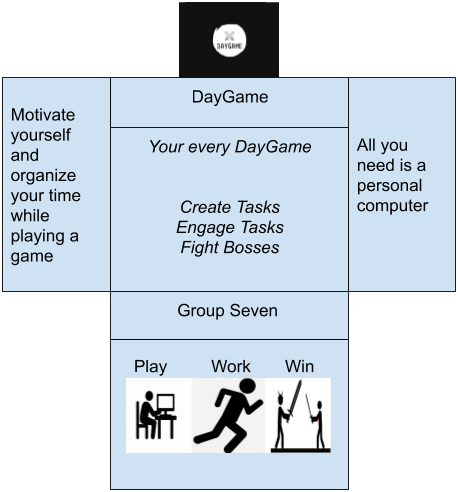
\includegraphics[width=1.0\textwidth]{./media/image2.png}
~
\end{figure}


%%%%%%%%%%%%%%%%%%%% Figure No: 2 Product In A Box Ends here %%%%%%%%%%%%%%%%%%%%

\begin{Center}

\end{Center}\par


\end{document}
